\documentclass[conference]{IEEEtran}
\IEEEoverridecommandlockouts
\usepackage{cite}
\usepackage{amsmath,amssymb,amsfonts}
\usepackage{algorithmic}
\usepackage{graphicx}
\usepackage{textcomp}
\usepackage{xcolor}
\usepackage{fancyhdr}
\usepackage{float}
\usepackage{subfigure}
\usepackage{pgfplots}
\pgfplotsset{compat=1.18}
\usepackage{tikz}
\usetikzlibrary{arrows.meta, positioning, shapes.geometric}
\usepackage{booktabs}
\usepackage{array}
\begin{document}
\title{Non-Planar Layering Strategy for Enhancing Buildability in Robotic 3D Concrete Printing with Cementitious Mortars\\
\thanks{* These authors contributed equally to this work.}
}
\author{
\IEEEauthorblockN{1\textsuperscript{st} Joaquin Velarde\textsuperscript{*}}
\IEEEauthorblockA{\textit{Faculty of Mechatronics Engineering} \\
\textit{Universidad Peruana de Ciencias Aplicadas (UPC)}\\
Lima, Per\'u \\
u20211b482@upc.edu.pe}
\and
\IEEEauthorblockN{1\textsuperscript{st} Gianpiero Huaricapcha\textsuperscript{*}}
\IEEEauthorblockA{\textit{Faculty of Mechatronics Engineering} \\
\textit{Universidad Peruana de Ciencias Aplicadas (UPC)}\\
Lima, Per\'u \\
u202113330@upc.edu.pe}
\and
\IEEEauthorblockN{2\textsuperscript{nd} Camila Sulen}
\IEEEauthorblockA{\textit{Faculty of Civil Engineering} \\
\textit{Universidad Peruana de Ciencias Aplicadas (UPC)}\\
Lima, Per\'u \\
camila.sulen@upc.edu.pe}
\and
\IEEEauthorblockN{3\textsuperscript{rd} Miguel Lara}
\IEEEauthorblockA{\textit{Faculty of Mechatronics Engineering} \\
\textit{Universidad Peruana de Ciencias Aplicadas (UPC)}\\
Lima, Per\'u \\
miguel.lara@upc.edu.pe}
}
\maketitle

\begin{abstract}
Extrusion-based 3D concrete printing (3DCP) has emerged as a transformative technology in the construction industry, enabling formwork-free fabrication of structural elements through layer-by-layer material deposition. However, the conventional planar layering strategy, where each layer is deposited as a horizontal plane, imposes fundamental limitations on the achievable geometries: staircase artifacts degrade surface quality on inclined surfaces, and buildability is severely constrained for overhanging or curved structures that require material deposition at angles beyond the self-supporting capacity of flat layers. While non-planar layering has been demonstrated in polymer-based fused deposition modeling (FDM) for improving surface finish, and tentatively explored in 3DCP for specific geometries, no study has systematically isolated the effect of the layering strategy with a paired comparison under identical material, nozzle, speed, and interlayer conditions on a cementitious mortar deposited by a six-DOF industrial robot. This paper presents the design and experimental methodology of such a comparison. The contribution is fourfold: (i) a parametric non-planar slicing pipeline implemented in Grasshopper/KUKA\textbar prc with a yield-stress-derived inclination constraint $\theta_{max}$, (ii) a closed-loop synchronization scheme between the tool-center-point (TCP) velocity and the volumetric flow rate of a progressive-cavity pump that compensates for mortar transit time through the hose, (iii) an explicit handling of kinematic singularities, orientation discontinuities, and TCP velocity drops on the KUKA robot, and (iv) a controlled experimental protocol that quantifies buildability ($N_{max}, \alpha_{max}, L_{max}$), surface roughness ($R_a, R_z$), and GD\&T deviations of planar versus non-planar specimens printed from the same nominal geometry. The test geometries (straight wall, inclined wall, overhang) are designed to expose the limitations of planar layering. The methodology is presented as a fully specified protocol; experimental results are part of the ongoing work and not reported here.
\end{abstract}

\begin{IEEEkeywords}
3D concrete printing, non-planar layering, buildability, cementitious mortars, robotic additive manufacturing, toolpath generation, surface quality
\end{IEEEkeywords}

\section{Introduction}

Extrusion-based 3D concrete printing (3DCP) is one of the most widely adopted digital fabrication methods for cementitious materials, enabling layer-by-layer construction of structural elements without conventional formwork \cite{bos_realities_2022}. The technology has advanced rapidly, with applications ranging from prefabricated architectural columns \cite{anton_3d_2021} to full-scale building structures. Despite this progress, the vast majority of current 3DCP processes rely on a planar layering strategy in which each deposited layer is a horizontal plane. While simple and well-understood, this approach imposes fundamental geometric limitations that constrain the design space of printed elements \cite{kiyani_influence_2025}.

The most prominent limitation of planar layering is the staircase effect: when the target geometry includes inclined or curved surfaces, the horizontal layers produce visible step artifacts whose severity increases as the surface angle approaches horizontal \cite{ahlers_3d_2019}. In addition to surface quality degradation, planar layering restricts buildability, that is, the capacity of the printed structure to maintain its shape under self-weight during fabrication, for geometries involving overhangs, cantilevers, or double curvature. In such cases, the horizontal layers must bridge unsupported spans, often leading to structural failure during printing \cite{bos_juxtaposing_2021, vele_enhancing_2024}. The buildability of 3DCP elements depends on the interplay of material properties (yield stress, structural build-up rate), process parameters (printing speed, layer height, nozzle standoff distance, interlayer time interval), and the geometric strategy of deposition \cite{wolfs_filament_2021, kiyani_influence_2025}. While extensive research has addressed the first two factors, the geometric strategy, specifically the shape of the layers themselves, has received comparatively little attention in the 3DCP literature.

Non-planar layering offers a fundamentally different approach: instead of constraining all layers to horizontal planes, the deposition paths follow curved or inclined surfaces that conform to the target geometry. In polymer FDM, Ahlers et al. \cite{ahlers_3d_2019} demonstrated that replacing the topmost planar layers with non-planar surfaces significantly improves surface finish quality while maintaining printability on standard three-axis printers. Their approach was integrated into an open-source slicer with collision checking, showing that the combination of planar and non-planar layers is both practical and effective for polymer materials. However, this strategy was designed for thermoplastic filaments with low self-weight and rapid solidification, conditions that do not hold for cementitious mortars.

In the context of 3DCP, Vele et al. \cite{vele_enhancing_2024} presented one of the few studies that directly addresses non-planar layering with concrete, demonstrating improved buildability for specific geometries. Their work provides initial evidence that curved layers can extend the geometric capabilities of concrete printing, but the experimental scope is limited to demonstrative geometries without a paired comparison against planar printing under identical material, nozzle, and speed conditions, and without a yield-stress-derived inclination constraint or a TCP-synchronized flow control loop.

Several complementary lines of work address print quality within the planar paradigm. Foteinopoulos et al. \cite{foteinopoulos_cement-based_2020} showed that the ratio of extrusion speed to print-head speed is the dominant factor for cement-based part quality; Wolfs et al. \cite{wolfs_filament_2021} mapped the influence of process parameters on filament geometry through CFD, identifying tearing and buckling regimes; and Csekei et al. \cite{csekei_optimization_2025} developed a volumetric feed-rate calibration for robotic FDM that achieved wall-thickness deviations below 0.07~mm. Filament-geometry prediction has been pursued through CFD \cite{COMMINAL2020106256}, PFEM \cite{reinold_extrusion_2022}, and deep-learning frameworks based on Fourier descriptors \cite{rizzieri_shapegen3dcp_2026}; Alhussain et al. \cite{alhussain_developing_2024} developed data-driven models for filament width, height, and contact width and explicitly noted their applicability to non-planar layer generation; Lao et al. \cite{lao_improving_2020} demonstrated machine learning-based extrudate control for surface finish. Nozzle and extrusion-system design have been advanced by Zhang and Sanjayan \cite{zhang_extrusion_2023, zhang_pumping-less_2024}, Lao et al. \cite{lao_variable-geometry_2021} (variable-geometry nozzle), and Yuan et al. \cite{yuan_real-time_2022} (real-time toolpath planning and extrusion control for variable-width 3DCP). Material characterization for buildability is treated in \cite{bos_juxtaposing_2021, ducoulombier_slugs-test_2021, bao_testing_2024, rehman_recommendations_2023, khan_impact_2024}, and GD\&T frameworks for 3DCP in \cite{xu_inspecting_2020}. On the digital-fabrication side, Kontovourkis and Tryfonos \cite{kontovourkis_integrating_2018} established the Grasshopper-to-industrial-robot workflow used in this paper, Breseghello and Naboni \cite{breseghello_toolpath-based_2022} demonstrated toolpath-based design as a structural variable, and Anton et al. \cite{anton_3d_2021} presented prefabrication of bespoke columns with process-specific parameter tuning.

\subsection{Scope of Contribution and Differentiation from Prior Work}
\label{subsec:scope}

To avoid ambiguity about what this paper does and does not claim to contribute, the scope is split into three blocks:

\textbf{Established evidence (taken from the literature, not contributed here).} Non-planar slicing in polymer FDM with collision checking \cite{ahlers_3d_2019}; CFD/PFEM prediction of 3DCP filament geometry \cite{COMMINAL2020106256, reinold_extrusion_2022}; the role of the extrusion-to-print speed ratio in planar 3DCP \cite{foteinopoulos_cement-based_2020}; the existence of a usable rheological window for printable mortars \cite{bos_juxtaposing_2021, bao_testing_2024}; the feasibility of non-planar layering in 3DCP for at least one geometry \cite{vele_enhancing_2024}; the GD\&T framework for evaluating 3DCP dimensional accuracy \cite{xu_inspecting_2020}.

\textbf{Proposed design (the methodological contribution of this paper).} (i)~A parametric non-planar slicing pipeline (Section~\ref{subsec:toolpath}) with a yield-stress-derived inclination constraint $\theta_{max}$ enforced as a hard limit in the slicer rather than as an empirical post-hoc rule; (ii)~a closed-loop TCP-velocity to flow-rate synchronization scheme (Section~\ref{subsec:sync}) that compensates explicitly for mortar transit time through the hose; (iii)~an explicit treatment of KUKA-specific singularities, orientation discontinuities, and TCP velocity drops (Section~\ref{subsec:kuka}); (iv)~a paired comparison protocol that isolates the effect of the layering strategy by holding material, nozzle geometry, speed, and interlayer time constant across planar and non-planar conditions on the same nominal geometry (Section~\ref{subsec:trials}).

\textbf{Experimental hypotheses (testable predictions, not results).} (H1)~For inclined and overhang geometries, non-planar layering produces strictly higher buildability ($N_{max}, \alpha_{max}, L_{max}$) than planar layering under identical process conditions. (H2)~For inclined geometries, non-planar layering produces lower arithmetic-mean roughness $R_a$ and lower maximum peak-to-valley $R_z$ than planar layering, with the gap widening as the inclination angle increases. (H3)~The TCP-synchronized flow control keeps the filament cross-section within $\pm 10\%$ of the planar baseline along three-dimensional paths, conditional on $v_{TCP} \geq 0.2 v_p$ along the path.

Table~\ref{tab:positioning} positions the proposed work along these axes against the most relevant prior work. Table~\ref{tab:maturity} reports the maturity of each pipeline component to make explicit where this paper builds on validated evidence and where it advances the frontier.

\begin{table*}[t]
\caption{Positioning of the proposed non-planar 3DCP strategy with respect to prior work}
\label{tab:positioning}
\centering
\renewcommand{\arraystretch}{1.15}
\begin{tabular}{@{}lccccc@{}}
\toprule
\textbf{Aspect} & \textbf{Planar 3DCP} & \textbf{Optimized planar} & \textbf{NP-FDM} & \textbf{NP-3DCP (prior)} & \textbf{This work} \\
                & (baseline) & \cite{foteinopoulos_cement-based_2020,csekei_optimization_2025} & \cite{ahlers_3d_2019} & \cite{vele_enhancing_2024} & \\
\midrule
Material                & Mortar                & Mortar                & Thermoplastic           & Mortar              & Mortar \\
Self-weight per layer   & High                  & High                  & Negligible              & High                & High \\
Layer geometry          & Horizontal            & Horizontal            & Curved (top only)       & Curved              & Curved, systematic \\
Hardware                & Gantry/robot          & Gantry/robot          & 3-axis                  & Robot               & 6-DOF KUKA \\
Nozzle orientation      & Fixed $\hat{\mathbf{z}}$ & Fixed $\hat{\mathbf{z}}$ & Fixed $\hat{\mathbf{z}}$ & Variable          & Aligned to $\hat{\mathbf{n}}_k$ \\
Flow rate control       & Constant              & SR-tuned              & Slicer-defined          & Limited             & TCP-velocity sync \\
$\theta_{max}$ rule     & N/A                   & N/A                   & Geometric/empirical     & Empirical           & Yield-stress derived \\
Comparison protocol     & N/A                   & SR sweep              & Surface finish          & Geometry-specific   & Paired planar/NP \\
GD\&T evaluation        & Common                & Common                & Not reported            & Not reported        & Applied to NP \\
\bottomrule
\end{tabular}
\end{table*}

\begin{table*}[t]
\caption{Experimental maturity matrix. Cells indicate the state of evidence for each pipeline component across paradigms.}
\label{tab:maturity}
\centering
\renewcommand{\arraystretch}{1.15}
\begin{tabular}{@{}lccccc@{}}
\toprule
\textbf{Pipeline component} & \textbf{Simulation} & \textbf{Polymer FDM} & \textbf{Planar 3DCP} & \textbf{NP-3DCP (prior)} & \textbf{This work} \\
\midrule
Non-planar slicing                   & Mature & Mature \cite{ahlers_3d_2019} & N/A & Initial \cite{vele_enhancing_2024} & Re-implemented in GH \\
Collision checking                   & Mature & Demonstrated \cite{ahlers_3d_2019} & Mature & Initial & GH + KUKA\textbar prc \\
6-DOF nozzle reorientation           & Mature & Not required & Demonstrated & Initial & Aligned to $\hat{\mathbf{n}}_k$ \\
Mortar rheology characterization     & Mature \cite{COMMINAL2020106256, reinold_extrusion_2022} & N/A & Mature \cite{bos_juxtaposing_2021, bao_testing_2024} & Limited & Vane + slugs-test \\
Flow rate--TCP synchronization       & Mature \cite{csekei_optimization_2025} & Standard & Established & Limited & Closed-loop Arduino + VFD \\
Buildability under inclination       & PFEM \cite{reinold_extrusion_2022} & N/A & Mature \cite{khan_impact_2024} & Limited & Paired $\theta_{max}$ sweep \\
Filament consistency on 3D path      & Predicted \cite{rizzieri_shapegen3dcp_2026,alhussain_developing_2024} & Demonstrated & Established & Limited & Measured on NP specimens \\
GD\&T evaluation                     & N/A & Common & Initial \cite{xu_inspecting_2020} & Absent & Applied to NP specimens \\
\bottomrule
\end{tabular}
\end{table*}

\subsection{Pipeline Overview}

Figure~\ref{fig:pipeline} summarizes the full pipeline from parametric CAD to evaluation. Each stage produces a checkpoint, geometric, kinematic, or material, before passing to the next; a failure at any checkpoint sends the path back to the upstream stage for local correction (e.g., layer flattening, orientation tolerance relaxation, recalibration).

\begin{figure*}[t]
\centering
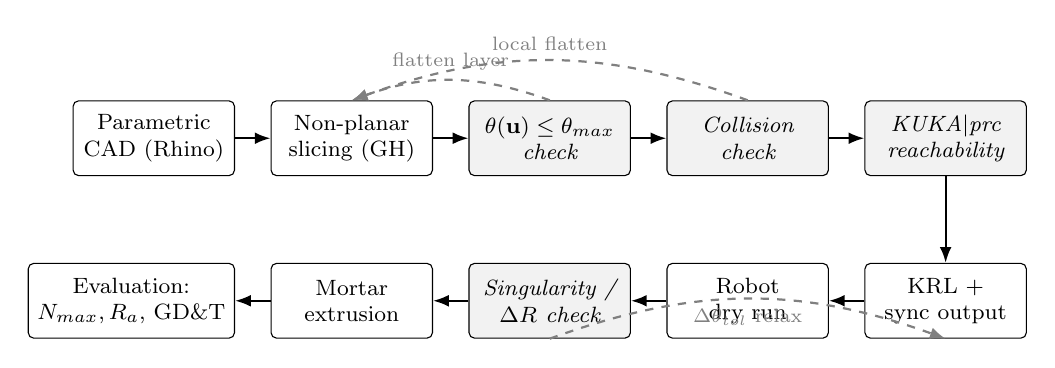
\begin{tikzpicture}[
    node distance=0.55cm and 0.45cm,
    box/.style={rectangle, draw, rounded corners=2pt, minimum height=0.95cm, minimum width=2.05cm, align=center, font=\footnotesize},
    checkbox/.style={rectangle, draw, rounded corners=2pt, fill=gray!10, minimum height=0.95cm, minimum width=2.05cm, align=center, font=\footnotesize\itshape},
    arrow/.style={-{Latex[length=2mm]}, thick},
    backarrow/.style={-{Latex[length=2mm]}, thick, dashed, gray}
]
\node[box] (cad) {Parametric\\CAD (Rhino)};
\node[box, right=of cad] (slice) {Non-planar\\slicing (GH)};
\node[checkbox, right=of slice] (theta) {$\theta(\mathbf{u}) \leq \theta_{max}$\\check};
\node[checkbox, right=of theta] (col) {Collision\\check};
\node[checkbox, right=of col] (prc) {KUKA\textbar prc\\reachability};

\node[box, below=1.1cm of prc] (krl) {KRL +\\sync output};
\node[box, left=of krl] (dry) {Robot\\dry run};
\node[checkbox, left=of dry] (sing) {Singularity /\\$\Delta R$ check};
\node[box, left=of sing] (ext) {Mortar\\extrusion};
\node[box, left=of ext] (eval) {Evaluation:\\$N_{max}, R_a$, GD\&T};

\draw[arrow] (cad) -- (slice);
\draw[arrow] (slice) -- (theta);
\draw[arrow] (theta) -- (col);
\draw[arrow] (col) -- (prc);
\draw[arrow] (prc.south) -- ++(0,-0.45) -| (krl.north);
\draw[arrow] (krl) -- (dry);
\draw[arrow] (dry) -- (sing);
\draw[arrow] (sing) -- (ext);
\draw[arrow] (ext) -- (eval);

\draw[backarrow] (theta.north) to[bend right=20] node[above, font=\scriptsize, gray]{flatten layer} (slice.north);
\draw[backarrow] (col.north) to[bend right=20] node[above, font=\scriptsize, gray]{local flatten} (slice.north);
\draw[backarrow] (sing.south) to[bend left=20] node[below, font=\scriptsize, gray]{$\Delta\theta_{tol}$ relax} (krl.south);
\end{tikzpicture}
\caption{End-to-end pipeline. Solid arrows: forward flow. Dashed arrows: feedback loops triggered by failed checkpoints. Gray boxes denote checkpoints; white boxes denote transformations.}
\label{fig:pipeline}
\end{figure*}

The objectives of this paper are therefore: (1)~to specify the parametric toolpath generation workflow with $\theta_{max}$ as a hard slicing constraint; (2)~to specify the TCP-flow synchronization architecture with transit-time compensation; (3)~to specify the KUKA-specific handling of singularities, orientation changes, and velocity drops; and (4)~to define the controlled experimental protocol that will be used to test hypotheses H1--H3.

\section{Methodology}

The methodology is structured in five stages: non-planar toolpath design (Section~\ref{subsec:toolpath}, proposed); mortar characterization including $\theta_{max}$ determination (Section~\ref{subsec:mortar}, proposed + established protocols); module-level validation (Section~\ref{subsec:validation}, established methods applied to the proposed pipeline); integrated printing trials (Section~\ref{subsec:trials}, proposed protocol); and evaluation (Section~\ref{subsec:eval}, established metrics applied to the proposed comparison).

\subsection{Non-Planar Toolpath Design}
\label{subsec:toolpath}

The toolpath generation for non-planar layers is implemented parametrically in Grasshopper (Rhinoceros 3D) using the KUKA\textbar prc plugin for robotic motion programming, following the parametric-to-robotic workflow established by Kontovourkis and Tryfonos \cite{kontovourkis_integrating_2018} and the toolpath-based design principles of Breseghello and Naboni \cite{breseghello_toolpath-based_2022}.

\subsubsection{Slicing Strategy}

Unlike conventional planar slicing, where the geometry is intersected with a series of horizontal planes spaced at the layer height $h_l$, the non-planar strategy generates layer surfaces that follow the local geometry of the target object. The approach proceeds as follows:

\begin{enumerate}
    \item \textbf{Base surface definition:} A reference surface $\mathcal{S}_0$ is defined, either as the build plate (for bottom-up printing) or as a curved surface conforming to the geometry.
    \item \textbf{Normal offset:} Successive layer surfaces $\mathcal{S}_k$ are generated by offsetting the previous surface $\mathcal{S}_{k-1}$ by the layer height $h_l$ along the local surface normal:
    \begin{equation}
        \mathcal{S}_k(\mathbf{u}) = \mathcal{S}_{k-1}(\mathbf{u}) + h_l \cdot \hat{\mathbf{n}}_{k-1}(\mathbf{u})
        \label{eq:offset}
    \end{equation}
    where $\mathbf{u}$ parameterizes the surface and $\hat{\mathbf{n}}_{k-1}$ is the unit normal of $\mathcal{S}_{k-1}$.
    \item \textbf{Contour extraction:} The intersection of each layer surface $\mathcal{S}_k$ with the target geometry yields the deposition contour $\mathcal{C}_k$.
    \item \textbf{Inclination constraint (hard slicing limit):} The local inclination angle $\theta$ of any layer surface, measured against the vertical, is bounded by the yield-stress-derived $\theta_{max}$ determined in Section~\ref{subsubsec:thetamax}:
    \begin{equation}
        \theta(\mathbf{u}) = \arccos\left(\hat{\mathbf{n}}_k(\mathbf{u}) \cdot \hat{\mathbf{z}}\right) \leq \theta_{max}
        \label{eq:angle_constraint}
    \end{equation}
    Points that violate Eq.~\ref{eq:angle_constraint} trigger a local flattening of the layer surface in a Gaussian neighborhood of radius $r_f = 2 w_f$, producing a hybrid planar/non-planar surface analogous to the strategy of Ahlers et al.~\cite{ahlers_3d_2019} but with a $\theta_{max}$ that is material-derived rather than geometric.
\end{enumerate}

\subsubsection{Nozzle Orientation}

For planar printing, the nozzle axis is aligned with the vertical direction $\hat{\mathbf{z}}$. In non-planar printing, the nozzle axis is aligned with the local surface normal $\hat{\mathbf{n}}_k(\mathbf{u})$ at each point along the deposition path. This requires the robot to continuously adjust the orientation of its end-effector, which is feasible with a six-DOF industrial robot but not with a standard three-axis gantry printer. The nozzle orientation at each path point $\mathbf{p}_i$ is specified as a rotation matrix $\mathbf{R}_i$ that aligns the tool $z$-axis with the surface normal:

\begin{equation}
    \mathbf{R}_i = f(\hat{\mathbf{n}}_k(\mathbf{p}_i), \hat{\mathbf{t}}_k(\mathbf{p}_i))
    \label{eq:orientation}
\end{equation}

\noindent where $\hat{\mathbf{t}}_k$ is the tangent direction of the deposition path at $\mathbf{p}_i$, used to resolve the rotational degree of freedom around the nozzle axis.

\subsubsection{Collision Checking}

Non-planar toolpaths introduce the risk of collision between the nozzle assembly and previously deposited material. Following the approach of Ahlers et al. \cite{ahlers_3d_2019}, collision checking is performed in Grasshopper by modeling the nozzle assembly as a simplified bounding volume (cylinder + bottom cone, plus a 5~mm safety margin) and testing for intersections with the accumulated print geometry at each layer. Path points that violate the collision constraint are flagged and the local layer surface is flattened with the same Gaussian rule as for $\theta_{max}$ violations. KUKA\textbar prc additionally performs robot-level collision checking and reachability analysis, ensuring that all programmed configurations are within the robot's joint limits and free of self-collision.

\subsubsection{Feed Rate Synchronization with TCP Velocity}
\label{subsec:sync}

In non-planar deposition, the effective TCP velocity $v_{TCP}$ varies along the path because the robot traverses a three-dimensional curve and necessarily decelerates near sharp orientation changes and near joint-velocity-limit margins. The volumetric flow rate $Q$ of the pump must be continuously matched to $v_{TCP}$ to maintain a consistent filament cross-section:

\begin{equation}
    Q(t) = v_{TCP}(t) \cdot w_f \cdot h_l
    \label{eq:flow_sync}
\end{equation}

\paragraph{Architecture} The synchronization loop consists of (i) the KUKA KR~C4 controller, which exposes the instantaneous TCP velocity through the \texttt{\$VEL\_ACT} system variable, (ii) a digital I/O bridge connecting the controller to an Arduino microcontroller via 24~V optoisolated channels, and (iii) a closed-loop pump driver based on a variable-frequency drive (VFD) controlling a progressive-cavity pump.

\paragraph{Signal and update rate} The TCP velocity setpoint is sent as an 8-bit PWM signal (0--255 mapped to 0--200~mm/s) updated at $f_s = 50$~Hz (period $T_s = 20$~ms). The Arduino converts this setpoint into a 0--10~V analog reference for the VFD. The control law is feed-forward with a static calibration curve $Q = g(\omega_{pump})$ obtained in the extrusion baseline of Section~\ref{subsubsec:extrusion-baseline}.

\paragraph{Latency budget} The end-to-end latency from a change in $v_{TCP}$ to the corresponding change in extruded flow is composed of: PWM update period (20~ms); Arduino processing ($<$1~ms); VFD response (50--100~ms depending on the ramp setting); and mortar transit time through the hose,
\begin{equation}
    t_{transit} = \frac{V_{hose}}{Q} = \frac{L_{hose} \cdot \pi D_{hose}^2 / 4}{Q},
    \label{eq:transit}
\end{equation}
which for $L_{hose} = 4$~m, $D_{hose} = 25$~mm and $Q = Q_{nom}$ gives $t_{transit} \approx 1.5$--3~s. The mortar transit time dominates the budget. It is compensated by a deterministic look-ahead in the KRL program: the pump setpoint sent at time $t$ corresponds to the $v_{TCP}$ scheduled at time $t + t_{transit}$, exploiting the fact that the toolpath is pre-computed and the controller has access to the full trajectory.

\paragraph{Calibration} Before each printing trial, a three-point calibration pass is executed at $v_p/2$, $v_p$, and $1.5 v_p$. Filament widths are measured at five points along each calibration line; if the deviation from the target $w_f$ exceeds 5\%, the curve $g(\omega_{pump})$ is refit.

\paragraph{Fault handling} If $v_{TCP}$ drops below $0.2 v_p$ (e.g., near a singularity or a sharp orientation reversal), the pump is held at its minimum stable speed to avoid backflow and segregation; the corresponding segment is logged and excluded from the evaluation in Section~\ref{subsec:eval}.

\subsubsection{Singularity, Orientation, and Velocity Handling on the KUKA Robot}
\label{subsec:kuka}

The six-DOF KUKA robot exhibits three behaviors that must be addressed explicitly in non-planar paths: kinematic singularities (wrist, shoulder, elbow), abrupt orientation changes between consecutive path points, and TCP velocity drops that break the synchronization assumption of Eq.~\ref{eq:flow_sync}.

\paragraph{Singularity avoidance} The non-planar toolpath is screened in KUKA\textbar prc using its built-in singularity detection on the inverse kinematics solution. Configurations within 5\textdegree{} of the wrist singularity ($A_5 \approx 0$) trigger a local re-orientation of the nozzle: instead of strictly $\hat{\mathbf{n}}_k$, the tool axis is allowed to deviate by up to $\Delta\theta_{tol} = 7$\textdegree{} from the surface normal so the inverse kinematics is well-conditioned. Path segments where no admissible configuration exists are flagged and the underlying layer surface is locally flattened with the same Gaussian rule used for $\theta_{max}$ violations.

\paragraph{Orientation smoothing} Adjacent path points whose nozzle orientations differ by more than $\Delta R_{max} = 15$\textdegree{} are interpolated with intermediate orientations using spherical linear interpolation (SLERP) so that the joint-space trajectory remains $C^1$-continuous. This avoids the sudden joint accelerations that the KUKA controller would otherwise compensate by reducing the TCP velocity, which in turn would break Eq.~\ref{eq:flow_sync}.

\paragraph{TCP velocity compensation} The KUKA controller is configured in \texttt{CONT} motion mode with an advance-run of 5 motion blocks, enabling look-ahead velocity profiling. The programmed $v_p$ is set 10\% below the joint-velocity limit of the slowest axis along the path, leaving margin for orientation transitions. The actual TCP velocity profile is logged through \texttt{\$VEL\_ACT} at 50~Hz; any segment where $v_{TCP}$ deviates more than 15\% from $v_p$ is excluded from the surface-quality and dimensional-accuracy analysis, isolating the effect of the layering strategy from the effect of robot-induced velocity variations.

\subsection{Test Geometries}
\label{subsec:geom}

Three test geometries are designed to systematically evaluate the effect of non-planar layering on buildability and surface quality, each exposing a specific limitation of planar printing:

\begin{enumerate}
    \item \textbf{Straight wall (baseline):} A single-filament-width wall of 400~mm length and target height of 20 layers, printed with conventional planar layers. This serves as the baseline for extrudability and dimensional consistency assessment, and establishes reference values for filament width, height, and buildability under the selected process parameters.

    \item \textbf{Inclined wall:} A wall with a progressive inclination from vertical (0\textdegree) to a target angle $\alpha_{target}$ (e.g., 30\textdegree{} from vertical). This geometry is printed twice: first with planar layers (producing visible stairstepping and potential buildability failure at high angles), and then with non-planar layers that follow the inclined surface. The comparison quantifies the effect of non-planar layering on both surface quality and maximum achievable inclination angle.

    \item \textbf{Overhang structure:} A wall with a horizontal overhang section extending beyond the base footprint. Planar layers cannot bridge the unsupported overhang beyond a critical length without support. Non-planar layers that curve gradually into the overhang distribute the self-weight load more favorably. This geometry tests the buildability limit of each strategy.
\end{enumerate}

Each geometry is defined parametrically in Grasshopper, enabling systematic variation of the inclination angle, overhang length, and number of layers.

\subsection{Mortar Characterization}
\label{subsec:mortar}

The cementitious mortar is characterized to establish its printability window and to determine the key parameters that govern non-planar deposition behavior. The rheometric and slump protocols below are established methods \cite{bos_juxtaposing_2021, ducoulombier_slugs-test_2021, bao_testing_2024}; the $\theta_{max}$ protocol of Section~\ref{subsubsec:thetamax} is proposed in this work.

\subsubsection{Mix Design}

The base mortar is a Portland cement-based mix designed for 3DCP, with a target rheological window consistent with extrudability and buildability requirements established in the literature: yield stress in the range of 300--900~Pa and plastic viscosity of 5--30~Pa$\cdot$s \cite{bos_juxtaposing_2021, bao_testing_2024}. The mix proportions (water-to-solid ratio, powder-to-sand ratio, and admixture dosages) are calibrated through preliminary flow-table tests following the correlation methodology of Bao et al. \cite{bao_testing_2024}.

\subsubsection{Rheological Measurements}

The rheological properties are measured using a rotational rheometer with a vane geometry. The following parameters are determined: static yield stress $\tau_{0,s}$, dynamic yield stress $\tau_{0,d}$, plastic viscosity $\mu_p$, and structural build-up rate $A_{thix}$ (Pa/s). Measurements are performed at rest times of 0, 5, 10, 15, 20, and 30 minutes to capture the time-dependent evolution relevant to the interlayer time intervals used in printing \cite{bos_juxtaposing_2021, rehman_recommendations_2023}. The yield stress at nozzle exit is additionally assessed using the slugs-test protocol of Ducoulombier et al. \cite{ducoulombier_slugs-test_2021}, providing a direct measure of the material state at the point of deposition.

\subsubsection{Critical Angle $\theta_{max}$ Determination}
\label{subsubsec:thetamax}

The maximum inclination angle $\theta_{max}$ at which a freshly deposited filament can be supported without slumping is the key parameter that connects the mortar rheology to the slicing constraint of Eq.~\ref{eq:angle_constraint}. It is determined through the following protocol:

\begin{enumerate}
    \item \textbf{Inclined substrates.} Rigid planar substrates pre-inclined at $\theta \in \{0, 10, 20, 30, 35, 40, 45\}$\textdegree{} relative to the horizontal.

    \item \textbf{Deposition.} A single filament of length $L = 200$~mm is printed on each substrate at nominal speed $v_p$ and flow rate $Q_0$, with the nozzle axis aligned with the local substrate normal.

    \item \textbf{Replication.} Five independent filaments per inclination from the same batch ($n_{batch} = 5$), repeated on three independent batches, for a total of $n_{total} = 15$ filaments per inclination angle.

    \item \textbf{Measurement windows.} Filament cross-sections are measured at $t = 30$~s, $t = 60$~s, and $t = 180$~s after deposition at three equidistant points along the filament length, using a digital caliper (0.01~mm) and a calibrated camera for cross-sectional profile capture.

    \item \textbf{Failure criteria (any one triggers failure of the filament).}
    \begin{itemize}
        \item Width gain $\Delta w_f / w_{f,0} > 15\%$ relative to the horizontal reference ($\theta = 0$\textdegree).
        \item Height loss $\Delta h_f / h_{f,0} > 15\%$ relative to the horizontal reference.
        \item Substrate-adhesion loss (delamination) over more than 10\% of the filament length.
        \item Lateral migration of the filament centerline by more than $0.25\, w_{f,0}$.
    \end{itemize}

    \item \textbf{Definition.} $\theta_{max}$ is the largest tested inclination at which the failure rate $p(\theta) < 1/15$. The failure rate per angle is reported with 95\% Wilson confidence intervals to propagate sample-size uncertainty into the slicing constraint.
\end{enumerate}

The four-criterion failure rule separates slump (gravity-driven cross-sectional deformation) from delamination (failure of substrate adhesion), both of which limit non-planar deposition with cementitious mortars. The resulting $\theta_{max}$ enters Eq.~\ref{eq:angle_constraint} as a hard constraint in the slicer.

\subsection{Module-Level Validation}
\label{subsec:validation}

Before executing integrated non-planar printing trials, each subsystem is validated independently.

\subsubsection{Toolpath Validation}

The non-planar toolpaths generated in Grasshopper are validated through: (1)~visual inspection of layer surfaces and contours in the Rhino viewport, (2)~collision analysis in KUKA\textbar prc with the nozzle bounding volume, and (3)~reachability and joint-limit analysis for all programmed robot configurations. Any path segments that violate constraints are automatically flagged and corrected through local flattening.

\subsubsection{Robot Dry Run}

The KUKA robot executes each non-planar toolpath without material extrusion (dry run) to verify: (1)~smooth trajectory execution without jerky motions or emergency stops, (2)~absence of joint-limit violations or singularity approaches, and (3)~consistency of TCP velocity along the path. The actual TCP velocity profile is logged from the robot controller through \texttt{\$VEL\_ACT} and compared against the programmed value.

\subsubsection{Extrusion Baseline}
\label{subsubsec:extrusion-baseline}

The mortar extrusion system (progressive cavity pump + nozzle) is calibrated by printing straight-line filaments at the nominal printing speed $v_p$ with planar deposition. The filament width $w_f$ and height $h_f$ are measured at five equidistant points along each filament using a digital caliper (0.01~mm resolution), following the measurement approach of Alhussain et al. \cite{alhussain_developing_2024}. The speed ratio $SR = v_e / v_p$ (extrusion velocity over printing speed) is verified to be above 0.8 as recommended by Foteinopoulos et al. \cite{foteinopoulos_cement-based_2020} for acceptable filament quality. The resulting curve $g(\omega_{pump})$ is the static feed-forward used by the synchronization loop of Section~\ref{subsec:sync}.

\subsection{Integrated Printing Trials}
\label{subsec:trials}

The experimental campaign consists of paired comparisons between planar and non-planar printing for each test geometry. Pairing is essential: each non-planar specimen is matched against a planar specimen printed from the same mortar batch, with the same nozzle, the same $v_p$, and the same interlayer time interval, so that the only varied factor is the layering strategy.

\subsubsection{Experimental Matrix}

Table~\ref{tab:exp_matrix} summarizes the experimental conditions. Each condition is replicated three times within batch and the experiment is repeated on three independent batches ($3 \times 3 = 9$ specimens per condition).

\begin{table}[htbp]
\caption{Experimental matrix for paired planar vs. non-planar comparison}
\label{tab:exp_matrix}
\centering
\begin{tabular}{@{}llll@{}}
\toprule
\textbf{ID} & \textbf{Geometry} & \textbf{Strategy} & \textbf{Variable} \\
\midrule
S1 & Straight wall  & Planar     & Baseline \\
S2 & Inclined wall  & Planar     & Angle: 15\textdegree, 30\textdegree \\
S3 & Inclined wall  & Non-planar & Angle: 15\textdegree, 30\textdegree \\
S4 & Overhang       & Planar     & Length: 20, 40~mm \\
S5 & Overhang       & Non-planar & Length: 20, 40~mm \\
S6 & Inclined wall  & Non-planar & $\theta_{max}$ sweep \\
\bottomrule
\end{tabular}
\end{table}

\subsubsection{Fixed Parameters}

The following parameters are held constant across all conditions to isolate the effect of the layering strategy: printing speed $v_p = 100$~mm/s, layer height $h_l = 10$~mm, nozzle standoff distance equal to layer height, nozzle outlet geometry (circular, $D_o = 20$~mm), interlayer time interval $t_{inter} = 30$~s, and mortar mix design. The pump feed rate is synchronized with the TCP velocity according to Eq.~\ref{eq:flow_sync}.

\subsubsection{Printing Protocol}

Each printing trial follows a standardized protocol: (1)~mortar mixing (3~min), (2)~pump priming and extrusion baseline verification (three-point calibration of Section~\ref{subsec:sync}), (3)~robot program upload and dry run confirmation, (4)~printing execution with synchronized video logging and \texttt{\$VEL\_ACT} logging at 50~Hz, and (5)~specimen marking and measurement within 30~min of printing completion.

\subsection{Evaluation Metrics}
\label{subsec:eval}

The printed specimens are evaluated against the hypotheses H1--H3 of Section~\ref{subsec:scope} using the following metrics.

\subsubsection{Buildability (tests H1)}

Buildability is assessed through two complementary measures \cite{bos_juxtaposing_2021, khan_impact_2024}: (1)~maximum number of stable layers $N_{max}$ deposited before structural failure (collapse, excessive deformation, or layer tearing), and (2)~maximum stable height $H_{max}$ measured from the build plate. For inclined and overhang geometries, buildability is additionally characterized by the maximum achieved inclination angle $\alpha_{max}$ and the maximum achieved overhang length $L_{max}$ without failure.

\subsubsection{Surface Quality (tests H2)}

Surface quality is evaluated through: (1)~surface roughness measurement along the outer face of printed walls using a contact profilometer, with arithmetic mean roughness $R_a$ and maximum peak-to-valley height $R_z$ as metrics, and (2)~qualitative visual assessment of stairstepping severity on a 1--5 scale by three independent evaluators (blinded to condition).

\subsubsection{Dimensional Accuracy}

The geometric precision of printed specimens is assessed using the GD\&T framework proposed by Xu et al. \cite{xu_inspecting_2020}. Printed specimens are digitized using a structured-light 3D scanner, and the resulting point cloud is registered against the nominal CAD geometry. Evaluated tolerances: flatness of wall surfaces, straightness of vertical edges, dimensional tolerance of wall thickness, and overall profile deviation from the target geometry.

\subsubsection{Filament Consistency in Non-Planar Deposition (tests H3)}

The cross-sectional geometry of filaments deposited at non-zero inclination angles is measured at representative points along the path. Filament width $w_f$, height $h_f$, and contact width $w_c$ are compared against the planar baseline values to quantify any degradation in filament consistency due to inclined deposition \cite{alhussain_developing_2024, wolfs_filament_2021}. Segments where $v_{TCP}$ deviated more than 15\% from $v_p$ are excluded as specified in Section~\ref{subsec:kuka}, so that the result reflects the synchronization scheme rather than residual robot dynamics.

\subsubsection{Statistical Analysis}

The experimental results are analyzed using a mixed-effects ANOVA with layering strategy (planar vs. non-planar) and geometry type as fixed factors and batch as a random factor, accommodating the paired and batch-nested structure of the experimental matrix. Post-hoc pairwise comparisons (Tukey HSD) are performed when significant main effects are found. The significance level is $\alpha = 0.05$. Effect sizes are reported as Cohen's $d$ for buildability and roughness metrics.

\section*{Acknowledgments}
The authors gratefully acknowledge the support of the Faculty of Engineering at Universidad Peruana de Ciencias Aplicadas (UPC) and the laboratory facilities provided for this research.

\bibliographystyle{IEEEtran}
\bibliography{references}

\end{document}